% %                                                                 aa.dem
% % AA vers. 9.1, LaTeX class for Astronomy & Astrophysics
% % demonstration file
%                                                       (c) EDP Sciences
%-----------------------------------------------------------------------
%
% \documentclass[referee]{aa} % for a referee version
%\documentclass[onecolumn]{aa} % for a paper on 1 column  
%\documentclass[longauth]{aa} % for the long lists of affiliations 
%\documentclass[letter]{aa} % for the letters 
%\documentclass[bibyear]{aa} % if the references are not structured 
%                              according to the author-year natbib style

\documentclass{aa}  

%
\usepackage{graphicx}
\usepackage{amsmath,amsfonts,amssymb}
\usepackage{natbib}

%%%%%%%%%%%%%%%%%%%%%%%%%%%%%%%%%%%%%%%%
\usepackage{txfonts}
\usepackage{xcolor}

\usepackage{blindtext}
%%%%%%%%%%%%%%%%%%%%%%%%%%%%%%%%%%%%%%%%
% \usepackage[options]{hyperref}
% To add links in your PDF file, use the package "hyperref"
% with options according to your LaTeX or PDFLaTeX drivers.
\usepackage{float}
%\usepackage{stfloats}
\usepackage{dblfloatfix}
\usepackage{afterpage}
\usepackage{ifthen}
\usepackage[morefloats=12]{morefloats}
\usepackage{threeparttable}

\usepackage{placeins}
\usepackage{multicol}
\usepackage[switch]{lineno}
\definecolor{linkcolor}{rgb}{0.6,0,0}
\definecolor{citecolor}{rgb}{0,0,0.75}
\definecolor{urlcolor}{rgb}{0.12,0.46,0.7}
\usepackage[breaklinks, colorlinks, urlcolor=urlcolor,
    linkcolor=linkcolor,citecolor=citecolor,pdfencoding=auto]{hyperref}
\hypersetup{linktocpage}
\usepackage{bold-extra}

\usepackage[nameinlink,capitalise]{cleveref}
\Crefname{section}{Sect.}{Sects.}
\Crefname{table}{Table}{Tables}
\Crefname{equation}{Eq.}{Eqs.}
\Crefname{appendix}{appendix}{appendices}
\makeatletter
\AddToHook{cmd/appendix/before}{\def\cref@section@alias{appendix}}
\makeatother

\usepackage{caption}
\usepackage{subcaption}

\DeclareRobustCommand{\ion}[2]{%
\relax\ifmmode
\ifx\testbx\f@series
{\mathbf{#1\,\mathsc{#2}}}\else
{\mathrm{#1\,\mathsc{#2}}}\fi
\else\textup{#1\,{\mdseries\textsc{#2}}}%
\fi}



\def\setsymbol#1#2{\expandafter\def\csname #1\endcsname{#2}}
\def\getsymbol#1{\csname #1\endcsname}

\def\Planck{\textit{Planck}}

\def\HeJT{$^4$He-JT}

\def\allearlypapers{\nocite{planck2011-1.1, planck2011-1.3, planck2011-1.4, planck2011-1.5, planck2011-1.6, planck2011-1.7, planck2011-1.10, planck2011-1.10sup, planck2011-5.1a, planck2011-5.1b, planck2011-5.2a, planck2011-5.2b, planck2011-5.2c, planck2011-6.1, planck2011-6.2, planck2011-6.3a, planck2011-6.4a, planck2011-6.4b, planck2011-6.6, planck2011-7.0, planck2011-7.2, planck2011-7.3, planck2011-7.7a, planck2011-7.7b, planck2011-7.12, planck2011-7.13}}

\def\alltwentythirteenresultspapers{\nocite{planck2013-p01, planck2013-p02, planck2013-p02a, planck2013-p02d, planck2013-p02b, planck2013-p03, planck2013-p03c, planck2013-p03f, planck2013-p03d, planck2013-p03e, planck2013-p01a, planck2013-p06, planck2013-p03a, planck2013-pip88, planck2013-p08, planck2013-p11, planck2013-p12, planck2013-p13, planck2013-p14, planck2013-p15, planck2013-p05b, planck2013-p17, planck2013-p09, planck2013-p09a, planck2013-p20, planck2013-p19, planck2013-pipaberration, planck2013-p05, planck2013-p05a, planck2013-pip56, planck2013-p06b, planck2013-p01a}}

\def\alltwentyfifteenresultspapers{\nocite{planck2014-a01, planck2014-a03, planck2014-a04, planck2014-a05, planck2014-a06, planck2014-a07, planck2014-a08, planck2014-a09, planck2014-a11, planck2014-a12, planck2014-a13, planck2014-a14, planck2014-a15, planck2014-a16, planck2014-a17, planck2014-a18, planck2014-a19, planck2014-a20, planck2014-a22, planck2014-a24, planck2014-a26, planck2014-a28, planck2014-a29, planck2014-a30, planck2014-a31, planck2014-a35, planck2014-a36, planck2014-a37, planck2014-ES}}

\newbox\tablebox    \newdimen\tablewidth
\def\leaderfil{\leaders\hbox to 5pt{\hss.\hss}\hfil}
\def\endPlancktable{\tablewidth=\columnwidth 
    $$\hss\copy\tablebox\hss$$
    \vskip-\lastskip\vskip -2pt}
\def\endPlancktablewide{\tablewidth=\textwidth 
    $$\hss\copy\tablebox\hss$$
    \vskip-\lastskip\vskip -2pt}
\def\tablenote#1 #2\par{\begingroup \parindent=0.8em
    \abovedisplayshortskip=0pt\belowdisplayshortskip=0pt
    \noindent
    $$\hss\vbox{\hsize\tablewidth \hangindent=\parindent \hangafter=1 \noindent
    \hbox to \parindent{$^#1$\hss}\strut#2\strut\par}\hss$$
    \endgroup}
\def\doubleline{\vskip 3pt\hrule \vskip 1.5pt \hrule \vskip 5pt}

\def\L2{\ifmmode L_2\else $L_2$\fi}
\def\dtt{\Delta T/T}
\def\DeltaT{\ifmmode \Delta T\else $\Delta T$\fi}
\def\deltat{\ifmmode \Delta t\else $\Delta t$\fi}
\def\fknee{\ifmmode f_{\rm knee}\else $f_{\rm knee}$\fi}
\def\Fmax{\ifmmode F_{\rm max}\else $F_{\rm max}$\fi}
\def\solar{\ifmmode{\rm M}_{\mathord\odot}\else${\rm M}_{\mathord\odot}$\fi}
\def\Msolar{\ifmmode{\rm M}_{\mathord\odot}\else${\rm M}_{\mathord\odot}$\fi}
\def\Lsolar{\ifmmode{\rm L}_{\mathord\odot}\else${\rm L}_{\mathord\odot}$\fi}
\def\inv{\ifmmode^{-1}\else$^{-1}$\fi}
\def\mo{\ifmmode^{-1}\else$^{-1}$\fi}
\def\sup#1{\ifmmode ^{\rm #1}\else $^{\rm #1}$\fi}
\def\expo#1{\ifmmode \times 10^{#1}\else $\times 10^{#1}$\fi}
\def\,{\thinspace}
\def\lsim{\mathrel{\raise .4ex\hbox{\rlap{$<$}\lower 1.2ex\hbox{$\sim$}}}}
\def\gsim{\mathrel{\raise .4ex\hbox{\rlap{$>$}\lower 1.2ex\hbox{$\sim$}}}}
\let\lea=\lsim
\let\gea=\gsim
\def\simprop{\mathrel{\raise .4ex\hbox{\rlap{$\propto$}\lower 1.2ex\hbox{$\sim$}}}}
\def\deg{\ifmmode^\circ\else$^\circ$\fi}
\def\pdeg{\ifmmode $\setbox0=\hbox{$^{\circ}$}\rlap{\hskip.11\wd0 .}$^{\circ}
          \else \setbox0=\hbox{$^{\circ}$}\rlap{\hskip.11\wd0 .}$^{\circ}$\fi}
\def\arcs{\ifmmode {^{\scriptstyle\prime\prime}}
          \else $^{\scriptstyle\prime\prime}$\fi}
\def\arcm{\ifmmode {^{\scriptstyle\prime}}
          \else $^{\scriptstyle\prime}$\fi}
\newdimen\sa  \newdimen\sb
\def\parcs{\sa=.07em \sb=.03em
     \ifmmode \hbox{\rlap{.}}^{\scriptstyle\prime\kern -\sb\prime}\hbox{\kern -\sa}
     \else \rlap{.}$^{\scriptstyle\prime\kern -\sb\prime}$\kern -\sa\fi}
\def\parcm{\sa=.08em \sb=.03em
     \ifmmode \hbox{\rlap{.}\kern\sa}^{\scriptstyle\prime}\hbox{\kern-\sb}
     \else \rlap{.}\kern\sa$^{\scriptstyle\prime}$\kern-\sb\fi}
\def\ra[#1 #2 #3.#4]{#1\sup{h}#2\sup{m}#3\sup{s}\llap.#4}
\def\dec[#1 #2 #3.#4]{#1\deg#2\arcm#3\arcs\llap.#4}
\def\deco[#1 #2 #3]{#1\deg#2\arcm#3\arcs}
\def\rra[#1 #2]{#1\sup{h}#2\sup{m}}
\def\page{\vfill\eject}
\def\dots{\relax\ifmmode \ldots\else $\ldots$\fi}
\def\WHzsr{\ifmmode $W\,Hz\mo\,sr\mo$\else W\,Hz\mo\,sr\mo\fi}
\def\mHz{\ifmmode $\,mHz$\else \,mHz\fi}
\def\GHz{\ifmmode $\,GHz$\else \,GHz\fi}
\def\mKs{\ifmmode $\,mK\,s$^{1/2}\else \,mK\,s$^{1/2}$\fi}
\def\muKs{\ifmmode \,\mu$K\,s$^{1/2}\else \,$\mu$K\,s$^{1/2}$\fi}
\def\muKRJs{\ifmmode \,\mu$K$_{\rm RJ}$\,s$^{1/2}\else \,$\mu$K$_{\rm RJ}$\,s$^{1/2}$\fi}
\def\muKHz{\ifmmode \,\mu$K\,Hz$^{-1/2}\else \,$\mu$K\,Hz$^{-1/2}$\fi}
\def\MJysr{\ifmmode \,$MJy\,sr\mo$\else \,MJy\,sr\mo\fi}
\def\MJysrmK{\ifmmode \,$MJy\,sr\mo$\,mK$_{\rm CMB}\mo\else \,MJy\,sr\mo\,mK$_{\rm CMB}\mo$\fi}
\def\microns{\ifmmode \,\mu$m$\else \,$\mu$m\fi}
\def\micron{\microns}
\def\muK{\ifmmode \,\mu$K$\else \,$\mu$\hbox{K}\fi}
\def\microK{\ifmmode \,\mu$K$\else \,$\mu$\hbox{K}\fi}
\def\muW{\ifmmode \,\mu$W$\else \,$\mu$\hbox{W}\fi}
\def\kms{\ifmmode $\,km\,s$^{-1}\else \,km\,s$^{-1}$\fi}
\def\kmsMpc{\ifmmode $\,\kms\,Mpc\mo$\else \,\kms\,Mpc\mo\fi}

\providecommand{\sorthelp}[1]{}


% Custom definitions
\newcommand{\mathsc}[1]{{\normalfont\textsc{#1}}}
\newcommand{\dv}[0]{\vec{d}}
\newcommand{\s}[0]{\vec{s}}
\newcommand{\M}[0]{\tens{M}}
\renewcommand{\P}[0]{\tens{P}}
\newcommand{\G}[0]{\tens{G}}
\newcommand{\B}[0]{\tens{B}}
\renewcommand{\a}[0]{\vec{a}}
\newcommand{\n}[0]{\vec{n}}
\renewcommand{\t}[0]{\vec{t}}
\def\Cosmoglobe{\textsc{Cosmoglobe}}
\def\cosmoglobe{\textsc{Cosmoglobe}}
\def\BeyondPlanck{\textsc{BeyondPlanck}}
\def\Planck{\textit{Planck}}
\def\planck{\textit{Planck}}
\def\NPIPE{NPIPE}
\def\npipe{NPIPE}
\def\FIRAS{\textit{FIRAS}}
\def\WMAP{\textit{WMAP}}
\def\COBE{\textit{COBE}}
\def\GAIA{\textit{Gaia}}
\def\gaia{\textit{Gaia}}
\def\Gaia{\textit{Gaia}}
\def\Ha{H$\alpha$}
\def\litebird{\textit{LiteBIRD}}
\def\WISE{WISE}
\def\AKARI{\textit{{AKARI}}}
\def\IRAS{\textit{{IRAS}}}
\def\nside{$N_{\mathrm{side}}$}
\def\wham{\textit{WHAM}}
% \newcommand{\cii}{\ensuremath{\mathsc{C\ ii}}}
\newcommand{\CII}{\ion{C}{ii}}
\newcommand{\cii}{\ion{C}{ii}}
% \newcommand{\CII}{\ensuremath{\mathsc{C\ ii}}}
\def\Commander{\texttt{Commander} }
\def\commanderthree{\texttt{Commander3} }

\def\Tcmb{\ifmmode T_\mathrm{CMB}\else $T_{\mathrm{CMB}}$\fi}
\def\Tcold{\ifmmode T_\mathrm{c}\else $T_{\mathrm{c}}$\fi}
\def\Thot{\ifmmode T_\mathrm{h}\else $T_{\mathrm{h}}$\fi}
\def\Tnear{\ifmmode T_\mathrm{near}\else $T_{\mathrm{near}}$\fi}
\def\scmb{\ifmmode s_\mathrm{CMB}\else $s_{\mathrm{CMB}}$\fi}
\def\squad{\ifmmode s_\mathrm{quad}\else $s_{\mathrm{quad}}$\fi}
\def\ssynch{\ifmmode s_\mathrm{s}\else $s_\mathrm{s}$\fi}
\def\sdust{\ifmmode s_\mathrm{d}\else $s_{\mathrm{d}}$\fi}
\def\ssdust{\ifmmode s_\mathrm{sd}\else $s_{\mathrm{sd}}$\fi}
\def\same{\ifmmode s_\mathrm{AME}\else $s_{\mathrm{AME}}$\fi}
\def\ssrc{\ifmmode s_\mathrm{src}\else $s_{\mathrm{src}}$\fi}
\def\sco{\ifmmode s_\mathrm{CO}\else $s_{\mathrm{CO}}$\fi}
\def\sff{\ifmmode s_\mathrm{ff}\else $s_{\mathrm{ff}}$\fi}
\def\gff{\ifmmode g_\mathrm{ff}\else $g_{\mathrm{ff}}$\fi}
\def\fsynch{\ifmmode f_\mathrm{s}\else $f_{\mathrm{s}}$\fi}
\def\fsd{\ifmmode f_\mathrm{sd}\else $f_{\mathrm{sd}}$\fi}
\def\fame{\ifmmode f_\mathrm{AME}\else $f_{\mathrm{AME}}$\fi}
\def\alphasrc{\ifmmode \alpha_\mathrm{src}\else $\alpha_{\mathrm{src}}$\fi}
\def\bcold{\ifmmode \beta_\mathrm{c}\else $\beta_{\mathrm{c}}$\fi}
\def\bhot{\ifmmode \beta_\mathrm{h}\else $\beta_{\mathrm{h}}$\fi}
\def\bnear{\ifmmode \beta_\mathrm{n}\else $\beta_{\mathrm{n}}$\fi}
\def\bsynch{\ifmmode \beta_\mathrm{s}\else $\beta_{\mathrm{s}}$\fi} 
\def\bsun{\ifmmode \beta_\mathrm{sun}\else $\beta_{\mathrm{sun}}$\fi} 
\def\nuzeros{\ifmmode \nu_{0,\mathrm{s}}\else $\nu_{0,\mathrm{s}}$\fi} 
\def\nuzeroff{\ifmmode \nu_{0,\mathrm{ff}}\else $\nu_{0,\mathrm{ff}}$\fi} 
\def\nuzerocold{\ifmmode \nu_{0,\mathrm{c}}\else $\nu_{0,\mathrm{c}}$\fi}
\def\nuzerohot{\ifmmode \nu_{0,\mathrm{h}}\else $\nu_{0,\mathrm{h}}$\fi}
\def\nuzeronear{\ifmmode \nu_{0,\mathrm{n}}\else $\nu_{0,\mathrm{n}}$\fi} 
\def\nuzeroame{\ifmmode \nu_{0,\mathrm{AME}}\else $\nu_{0,\mathrm{AME}}$\fi} 
\def\nuzerosd{\ifmmode \nu_{0,\mathrm{}}\else $\nu_{0,\mathrm{sd}}$\fi} 
\def\nuzerosrc{\ifmmode \nu_{0,\mathrm{src}}\else $\nu_{0,\mathrm{src}}$\fi} 
\def\nup{\ifmmode \nu_{\mathrm{p}}\else $\nu_{\mathrm{p}}$\fi} 
\def\alphasd{\ifmmode \alpha_{\mathrm{sd}}\else $\alpha_{\mathrm{sd}}$\fi} 
\def\Te{\ifmmode T_{\mathrm{e}}\else $T_{\mathrm{e}}$\fi} 
\def\kB{\ifmmode k_\mathrm{B}\else $k_{\mathrm{B}}$\fi} 

\newcommand{\RS}[1]{\textcolor{red}{RS: #1}}

\definecolor{darkpastelgreen}{rgb}{0.01, 0.75, 0.24}
\usepackage[normalem]{ulem} % enables \sout to strikeout text
\newcommand{\KG}[1]{\textcolor{darkpastelgreen}{(KG: #1)}}

\begin{document} 
\linenumbers

%\title{\bfseries{\Cosmoglobe\ DR2. VI. High-resolution templates of hot and cold thermal dust emission derived from Planck HFI}}
\title{\bfseries{\Cosmoglobe\ DR2. VI. Disentangling hot and cold thermal dust emission with Planck HFI}}
%\title{\bfseries{\Cosmoglobe\ DR2. VI. Decomposing thermal dust emission in Planck HFI }}
%\title{\bfseries{\Cosmoglobe\ DR2. VI. High-resolution decomposition of hot and cold thermal dust emission derived from Planck HFI}}


   %This author list corresponds to \title{Author list for L04\_CMB\_Foregrounds\_Extraction}
%Prepared by M. Lopez-Caniego (Marcos.Lopez.Caniego@sciops.esa.int), ESAC/ESA
%This version is from Thu Jul 12 18:11:48 2018 CET
%\subtitle{There are 152 co-authors in this list}
\newcommand{\oslo}[0]{1}
%\newcommand{\MIT}[0]{2}
\newcommand{\milanoA}[0]{2}
\newcommand{\milanoB}[0]{3}
\newcommand{\milanoC}[0]{4}
\newcommand{\triesteB}[0]{5}
\newcommand{\planetek}[0]{6}
\newcommand{\princeton}[0]{7}
\newcommand{\jpl}[0]{8}
\newcommand{\helsinkiA}[0]{9}
\newcommand{\helsinkiB}[0]{10}
\newcommand{\nersc}[0]{11}
\newcommand{\haverford}[0]{12}
\newcommand{\mpa}[0]{13}
\newcommand{\triesteA}[0]{14}
\newcommand{\iia}[0]{2}

\author{\small
J.~R.~Eskilt\inst{\oslo}\thanks{Corresponding author: J.~R.~Eskilt; \url{j.r.eskilt@astro.uio.no}}
\and
K.~Lee\inst{\oslo}
\and
D.~J.~Watts\inst{\oslo}
\and
S.~Nerval\inst{\oslo}
\and
et al.
}
\institute{\small
        Institute of Theoretical Astrophysics, University of Oslo, Blindern, Oslo, Norway \goodbreak
}



   % Shortened title, author list for top of page 
   \titlerunning{Disentangling cold and hot dust with HFI}
   \authorrunning{Sullivan et al.}

   \date{\today} 
   
   \abstract{
	   We present a four-component high-resolution model of thermal dust emission for microwave and infrared frequencies derived from \textit{Planck} HFI, WHAM and \textit{Gaia}. This model is inspired by a joint low-resolution template-based analysis of \textit{Planck} HFI and \textit{COBE}-DIRBE data presented in \citet{CG02_05}, and this resulting high-resolution model forms the basis for the thermal dust model employed in the \textsc{Cosmoglobe} DR2 reanalysis of \textit{COBE}-DIRBE. The four dust components correspond to different semi-independent physical effects, referred to as ``cold dust'', ``hot dust'',  ``nearby dust'', and ``\Ha\ correlated dust''. The \Ha\ dust is a dust extinction component, and has a negative amplitude in the \textit{Planck} HFI bands. The spatial distributions of the nearby dust and \Ha\ dust components are defined by a \textit{Gaia} 3D extinction model \citep{edenhofer:2024} and the Wisconsin \Ha\ mapper (WHAM; \citealp{wham:2003,2016WHAM}), respectively, while the hot and cold dust components are fit freely pixel-by-pixel to the \textit{Planck} HFI data. 
       %The spectral energy densities (SEDs) of all four components are modelled in terms of modified blackbody (MBB) spectra with a free global temperature, $T$, and spectral index, $\beta$, both of which are fitted globally across the sky. Thus, this dust model has ten global sky parameters (two SED parameters for each dust component plus two global template amplitude parameters) and two amplitudes per pixel, one each for the hot and cold dust; in contrast, previous \textit{Planck} HFI dust models have typically assumed spatially varying MBB temperatures and spectral indices, resulting in three degrees of freedom per pixel. 
       We use a parameter grid search (for global parameters) coupled to a Bayesian Gibbs sampler (for per-pixel parameters) to fit this model to \textit{Planck} HFI data. The fiducial MBB temperature for the hot and cold dust components are $T_{\mathrm{h}} = 30\pm3\,\mathrm{K}$ and $T_{\mathrm{c}} = 11\pm1\,\mathrm{K}$, and the corresponding fiducial spectral indices are $\beta_{\mathrm{h}}\ge1.75$ and $\beta_{\mathrm{c}}=1.85\pm0.10$, respectively. In agreement with the low-resolution template fit analysis of \citet{CG02_05}, we find that the hot dust component is strongly correlated with the FIRAS \ion{C}{ii} map, while the cold dust component is strongly correlated with the HI4PI \ion{H}{i} map.
 Despite its fewer degrees of freedom per pixel compared to the \textit{Planck} 2018 legacy dust model, we find that this new model performs competitively in terms of overall residuals, capturing between 98.5 and 99.9\,\% of the full-sky dust RMS for all channels between 100 and 857\,GHz. %When fitting a spatially varying 3-parameter MBB model to the new four-component dust model with isotropic SEDs, we find  similar spatial distributions of $T$ and $\beta$ to those of the official \textit{Planck} analysis. 
 We conclude that this new model represents both a statistically more efficient summary of thermal dust in the microwave and far-infrared regimes, as well as a physically more realistic decomposition of the sky.
 %, compared to the traditional 3-parameter MBB model, due to its strong correlations with well-defined \ion{C}{ii} and \ion{H}{i} line emission tracers. 
 Finally, we expect that the novel templates of hot and cold dust emission presented in this paper may form a key component in future temperature and polarization measurements for projects such as Simons Observatory and \litebird, where high-precision measurements of the dust will be critical for constraining $B$-mode CMB polarization. 
   }
   \keywords{ISM: general - Cosmology: observations, diffuse radiation - Galaxy: general}

   \maketitle
% \setcounter{tocdepth}{2}

% \tableofcontents
   
% INTRODUCTION
%-------------------------------------------------------------------
\section{Introduction}
Observing the Universe through a screen of foregrounds offers opportunities for both discovery and frustration \citep{Planck2018xii,planck2016-l04,bicep2_2014}. The foregrounds ultimately complicate our understanding of the backgrounds, and when poorly understood, lead to increased uncertainties or even misinterpretations. A better understanding of the foregrounds allows us to uncover the physics permeating matter on all scales, from within our solar system \citep[e.g.,][]{K98}, to the Milky Way \citep[e.g.,][]{planck2014-a12}, to distant galaxies \citep[e.g.,][]{planck2014-XXV,planck2014-XXVI,planck2011-5.2a}, while simultaneously allowing us to better observe the far away signals of the Cosmic Microwave Background (CMB; \citealp{penzias:1965}) and the Cosmic Infrared Background (CIB; \citep{partridge1967}), among others. Of particular interest to this paper and the cosmology community at large is the composition of thermal dust \citep[e.g.,][]{planck2013-p06b,Hensley2023}. Thermal dust represents a significant noise contribution to future measurements of primordial polarization $B$-modes \citep[][]{Bicep2018limit}, predicted to have been generated by gravitational waves during inflation \citep, which is the primary goal of several ongoing or upcoming CMB experiments \citep{litebird2022,SO2019}. 

Aside from the aforementioned dust, the Milky Way contains gas (generating emission lines such as singly ionized carbon (\ion{C}{ii}), hydrogen emission lines such as \Ha, neutral hydrogen (\ion{H}{i}), carbon monoxide (CO) and many more), stars, spinning dust, ions and electrons (interacting with magnetic fields to produce synchrotron and free-free radiation) and dark matter (only thus far interacting gravitationally). Each of these foregrounds trace relevant regions of the Milky Way and the interstellar medium (ISM). Since dust and gas live side-by-side, it is natural that one may trace the other, and indeed it is known that the neutral hydrogen signature (as observed by, e.g., HI4PI, \citealt{HI4PI2016}) and CO \citep{dame2001} trace cold dust. Another observable we can use is the reddening or extinction measurements of starlight, which occurs when their light passes through dust regions \citep[e.g.,][]{lenz:2017,lallement:2022,edenhofer:2024}. Finally, as recently shown by \cite{CG02_05}, the \ion{C}{ii} emission lines, as measured by COBE-FIRAS \citep{mather:1994}, trace hot dust regions. Before \cite{CG02_05} it was not known to us that \ion{C}{ii} could be used directly as a high-precision dust tracer; however, as it is expected to be present in hot regions of the Milky Way, it is not unexpected that this acts as a tracer for the hot dust.\footnote{It has also been hypothesized that dust may be responsible for the \ion{C}{ii} deficit in luminous-FIR galaxies \citep{2020CII,2017Herschel_FIR_CII}.} 

The dust in the Milky Way will act to absorb radiation at frequencies close to its particle size and re-emit as an imperfect blackbody. Historically, this has been modeled with a modified blackbody spectrum (MBB) characterized by a temperature, $T$, and a `tilt' to the spectrum, called the spectral index and denoted by $\beta$. These, along with an amplitude ($\vec{a}$), define how much radiation at a particular frequency, $\nu$, is produced (see \citet{Hensley2023} for a recent review of dust and the interstellar medium). During the \planck\ analysis the dust in the Milky Way was often modelled with a single modified blackbody fit for each pixel, or direction, in the sky. However, it is known that there are different dust populations \citep{finkbeiner1999}, and with enough data it should be possible to make distinct templates modelling each independently. A significant challenge that \planck\ faced in their analysis was that there was insufficient data to distinguish these populations; in particular, there is a clear degeneracy between the dust temperature and the dust spectral index maps \citep{juvela:2012,planck2014-a12}.

In the current paper, we revisit the model introduced by \citet{CG02_05}. In that paper, the authors found that thermal dust emission in the \Planck\ HFI and \COBE-DIRBE data on large angular scales could be well described by a sum of five external dust templates, namely 1) COBE-FIRAS \ion{C}{ii}; 2) HI4PI \citep{HI4PI2016}; 3) \Gaia\ extinction \citep{edenhofer:2024}; 4) WHAM \Ha\ \citep{wham:2003,2016WHAM}; and 5) CO\,$J$=$1-0$ \citep{dame2001}. They furthermore noted that the \ion{C}{ii} map template was associated with a higher temperature than the HI4PI and CO templates; that the nearby \Gaia\ extinction template corresponded to an intermediate temperature; and that the \Ha\ template was observed in absorption (i.e., having a negative template amplitude). The main goal of the current paper is to establish a corresponding  multi-component model for \Planck\ HFI at full angular resolution. Since the FIRAS \ion{C}{ii} map has a very low angular resolution of $7^{\circ}$ FWHM, this means that the morphology of the hotter dust component has to be derived directly from the \Planck\ data, rather than traced by an already existing template. Furthermore, the HI4PI and Dame et al.\ templates also have issues that prevent their direct use as a template (e.g., lower resolution and/or incomplete sky coverage). The key operational step in the current analysis is therefore to establish separate maps of cold and hot dust directly from the \Planck\ HFI data themselves. Since we do not use a template for the hot and cold dust, this also acts as a confirmation of the effects seen in \cite{CG02_05}, as the \planck\ data set is independent of the DIRBE data set, both in terms of the frequencies observed and the telescope. Finding a cold and hot dust component tightly tracing the \ion{H}{i} and \ion{C}{ii} gas acts as a strong confirmation of the results previously shown. 

Physically, each of these dust components should represent semi-independent dust populations. While in a perfect world we would have enough data to smoothly map an entire range of temperatures and dust populations, having two dust temperatures, and the two templates for dust populations nearby to us, and dust in \Ha\ emission regions allows for a good compromise, without allowing too many free parameters. We do not discuss here what these dust populations expressly represent, and leave such an analysis to future work. 

Following \cite{CG02_05}, we adopt the maps produced by \cite{edenhofer:2024} with \textit{Gaia} data \citep{gaia:2016} to trace nearby dust in the Milky Way, and the \Ha\ map produced by the Wisconsin H-$\alpha$ mapper (WHAM) \citep{wham:2003,2016WHAM} to trace a sub-dominant level of dust absorption. These two data sets are used as templates, fixing the relative amplitudes between pixels, but allowing the overall amplitudes of the maps, as well as the temperature and spectral indices, to vary globally. We introduce two additional dust components, here called the hot and the cold dust, which have freely varying amplitudes per pixel, but a global temperature and spectral index. Compared to the previous \planck\ analysis, which had three free parameters per pixel ($\vec{T}$,$\vec{\beta}$ and $\vec{a}$ at each pixel), we instead have ten global parameters, with only two free parameters per pixel, the hot and cold dust amplitudes. At high resolutions (like those seen here for \planck\ HFI) this represents a significant reduction in the number of model parameters, and has the additional advantage of producing clear correlations between the cold dust and the HI4PI maps (a known cold dust tracer), and the hot dust and \ion{C}{ii}. 

This paper is one of seven companion papers from the \cosmoglobe\ data release 2 \citep[DR2;][]{CG02_01} reanalyzing the \COBE-DIRBE data \citep{hauser1998}. Of particular interest for this release is new constraints on the spectrum of the CIB \citep{CG02_03}, and better constraints on all foregrounds ranging from the microwave to the infrared, including zodiacal light \citep{CG02_02} and stars \citep{CG02_04}. 
%paragraph mimicking the Dust05 
In a companion dust paper, by \cite{CG02_05}, we perform a linear regression analysis of \planck\ HFI 353-857~GHz and DIRBE 3.5-100~$\mu$m data to a five template dust model with minimal assumptions. That analysis clearly demonstrates that there are distinct dust populations that can be modelled independently with sufficient data sets at a wide range of frequencies, and revealed the new dust tracer, the \ion{C}{ii} line emission, tracing hot dust. 
 Building off of that work, in the current paper we perform a Bayesian analysis of the \planck\ HFI data, deriving high-resolution templates of \ion{H}{i} and \ion{C}{ii} correlated dust components, as well as the \Ha\ and nearby dust template fits. Finally, in \cite{CG02_07} this new dust model is applied to the \COBE-DIRBE data. 

%what is gonna happen in this paper
The rest of the paper is organized as follows. In \cref{sec:data} we discuss the data sets we use for this analysis. We next discuss the sky and data model in \cref{sec:skymodel}. In \cref{sec:method} we discuss our methodology, primarily the Gibbs sampling and grid search tests, along with the optimization strategy used for the grid search. In \cref{sec:results} we present the best fit results for our new thermal dust model. In \cref{sec:gof} we discuss the goodness of fit of the model, and in \cref{sec:correlations} the correlations with external line emission maps. In \cref{sec:mbb} we compare to the previous \planck\ results and show the MBB fit to the multi-component dust model. Finally, in \cref{sec:conc} we present our conclusions. In \cref{app:RMSScale}, \cref{app:dustTemplates}, \cref{app:residuals}, \cref{app:GridSearchTests} and \cref{app:dustCharacterization} we include supplementary details regarding the data preprocessing, dust templates, residuals, the grid search, and the dust characterization for clarity.

\begin{figure}
	\centering
	\includegraphics[width=0.9\linewidth]{figures/all_masks.pdf}
	\caption{All masks used for different stages of the analysis. \emph{HFI:} Mask used during the HFI Gibbs sampling routine for the monopoles, dipoles and $\chi^2$ evaluation. \emph{FIRAS:} Mask used during the FIRAS Gibbs sampling routine for the monopoles, dipoles and $\chi^2$ evaluation. \emph{857 GHz:} Mask used during the 857~GHz gain Gibbs sampling routine. \emph{$\chi^2$:} Mask used to compare the $\chi^2$ in the grid search.}
	\label{fig:all_masks}
\end{figure}


\section{Data}
\label{sec:data}
Building on the work of \cite{CG02_05}, this analysis uses the \planck\ PR4 data (\cref{sec:planckhfi}), several FIRAS maps (\cref{sec:firas}), and additional ancillary data (\cref{sec:otherdata}) to constrain a new high resolution four component dust model. We discuss our masks in \cref{sec:masks}. 

\subsection{\Planck\ HFI}
\label{sec:planckhfi}
The \planck\ PR4 (also known as \npipe) maps are the final \planck\ data release, improving on previous data releases by jointly analyzing the low-frequency instrument (LFI) and the  high-frequency instrument (HFI) data in a single pipeline, in addition to numerous other improvements (for details see \cite{planck2020-LVII}). 
For this analysis we use the single-horn HFI maps, chosen because HFI offers strong constraining power on the dust and the single-horn maps are able to better control the gain fluctuations and model components such as the CO-emission.\footnote{The 100~GHz and 143~GHz maps are at a HEALPix\footnote{\url{http://healpix.sourceforge.net/}} pixelization \citep{healpix,Zonca2019} \nside\ of 2048, the other frequencies are at an \nside\ of 4096.} Specifically we use the 100--\{1-4\}, 143--\{1-7\}, 217--\{1-8\}, 353--\{1-8\}, 545--\{1,2,4\} and 857--\{1-4\}.\footnote{The 143-8 and 545-3 maps were never released by the \planck\ collaboration due to non-Gaussian noise in the data, known as random telegraphic signal \citep{planck2013-p03}.}
In a pre-processing step we correct all maps for the zodiacal light emission, using the \Planck\ PR2 zodiacal light model \citep{planck2014-a09, planck2013-pip88, maris2006c}, and apply a correction for the CIB to the 857, 545 and 353 GHz maps from the GNILC CIB results \cite{planck2016-XLVIII}.
We apply a scaling correction to the root-mean squared (RMS) maps, such that the tail of the map power spectra match the white-noise level from the RMS maps.\footnote{The published single horn frequency RMS maps have known residual offsets from the analysis pipeline, evident when comparing the map and RMS power-spectra.} These scaling values can be found in \cref{app:RMSScale}.


\subsection{FIRAS}
\label{sec:firas}
FIRAS was a cosmology telescope, launched in 1989 as part of the COBE satellite mission, with the goal of measuring the blackbody spectrum of the CMB to unprecedented precision \citep{fixsen1997}. The FIRAS maps have very low calibration uncertainties, and so we use them to help calibrate the map amplitudes. The FIRAS 857, 1251, 1809, 2081, 2135 and 2802~GHz maps are used for this analysis in conjunction with the HFI maps. 

\subsection{Ancillary data}
\label{sec:otherdata}
The nearby dust relative amplitudes are fixed to the \GAIA-based dust extinction template produced by \citet{edenhofer:2024}, which covers distances up to 1.25~kpc. This primarily uses \GAIA\ distances and extinction estimates to build a 3D map of the nearby dust from \citet{2023Zhang} and \GAIA\ \citep{2019GAIA,2023gaia}, which also leverages the two Micron All Sky Survey (2MASS,\cite{2006AJ_2mass}), the Wide-field Infrared Survey Explorer (WISE and unWISE; \cite{allwise_ES,2010AJ_wise}), the Large sky Area Multi-Object fibre Spectroscopic Telescope (LAMOST; \cite{2023yCatp038060301X_lamost,2022A&A_lamost,2022ApJS_lamost,2022yCat_lamost}). We use the total integrated dust map as our model in this analysis. 
Additionally, we use the Wisconsin H-$\alpha$ Mapper (WHAM) data \citep{wham:2003,2016WHAM} as a template for the \Ha\ correlated dust and the results from \citep{CG02_05} as the fiducial values for the \Ha\ MBB, since we find that it is poorly constrained by the \planck\ bands (see \cref{sec:results}). As with DIRBE, the \Ha\ dust is a small extinction component in the \Planck\ bands.  
When considering our summary statistics in \cref{sec:correlations} we compare the new dust templates with the 157.7$\mu$m \ion{C}{ii} line emission as measured by the FIRAS \ion{C}{ii} map, available on the LAMBDA\footnote{\url{lambda.gsfc.nasa.gov}} website, and to the HI4PI data \citep{HI4PI2016}. 

\subsection{Masks}
\label{sec:masks}
When computing the $\chi^2$ for the grid search (see \cref{sec:statistics}) we apply a mask to remove the extreme outliers in the $\chi^2$ map, as can be seen in yellow in \cref{fig:all_masks}, this has an $f_\mathrm{sky}$ of 99\% (masking only 1\% of the sky).
During the Gibbs sampling (see \cref{sec:sampling}), we apply a 30 degree galactic plane mask to the FIRAS maps when computing monopole and dipole estimates (representing an $f_\mathrm{sky}$ of 50\%), and a large galactic cut (of areas with the largest foregrounds) to the HFI maps with an $f_\mathrm{sky}$ of 48\%, as can be seen in dark and light purple in \cref{fig:all_masks}. When estimating the gain for the 857~GHz maps we employ a small mask of $f_\mathrm{sky}$ of 95\%, as seen in orange in \cref{fig:all_masks}. The component estimation (as discussed in \cref{sec:skymodel}) was done using the full sky.

\section{Data model}
\label{sec:skymodel}
The data model for this analysis can be written as
\begin{align}
    \vec{d}=&\mathsf{G}\left[\mathsf{B}\sum_s \mathsf{M}_{s}\vec{a}_{s}\right]+\vec{n}\nonumber\\
    \equiv & \vec{s}+ \vec{n},
\label{equ:dataModel}
\end{align}
where $\mathsf{G}$ is the instrumental gain matrix for each detector, $\mathsf{B}$ the instrumental beam convolution, $\mathsf{M}_{s}a_{s}$ is the foregrounds mixing matrix which extrapolates the sky component $s$ to the given frequency (including bandpass and the spectral shape of the particular component) and amplitudes $\vec{a}_{s}$ per pixel for the various sky components ($s$), and $\vec{n}$ is the noise. 

The \planck\ HFI bands contain several relevant sky components in addition to dust, such as free-free, CO, and the CMB. 
 As such, the sky model used for this analysis may be written as a vector per pixel
\begin{align}
    \vec{s}_\nu=&u_\nu 
    \left[\vphantom{\left(\frac{\nu}{\nu_\mathrm{d}}\right)^{\beta_\mathrm{d}+1}}\vec{a} _\mathrm{CMB}\gamma(\nu) \right. &\mathrm{(CMB)} \nonumber \\
    &+\vec{t}_\mathrm{ff}\left(\frac{\nu_{0,\mathrm{ff}}}{\nu}\right)^2\frac{g_\mathrm{ff}(\nu;T_\mathrm{e})}{g_\mathrm{ff}(\nu_{0,\mathrm{ff}};T_\mathrm{e})} & \textrm{(Free-free)}\nonumber \\
    &+\vec{a}_\mathrm{c}\left(\frac{\nu}{\nu_\mathrm{c}}\right)^{\beta_\mathrm{c}+1}\left(\frac{e^{h\nu_\mathrm{c}/k_\mathrm{B}T_\mathrm{c}}-1}{e^{h\nu/k_\mathrm{B}T_\mathrm{c}}-1}\right) &\textrm{(Cold\ dust)}\nonumber \\
    &+\vec{a}_\mathrm{h}\left(\frac{\nu}{\nu_\mathrm{h}}\right)^{\beta_\mathrm{h}+1}\left(\frac{e^{h\nu_\mathrm{h}/k_\mathrm{B}T_\mathrm{h}}-1}{e^{h\nu/k_\mathrm{B}T_\mathrm{h}}-1}\right) &\textrm{(Hot\ dust)}\nonumber \\
    &+a_\mathrm{near}\vec{t}_\mathrm{near}\left(\frac{\nu}{\nu_\mathrm{near}}\right)^{\beta_\mathrm{near}+1}\left(\frac{e^{h\nu_\mathrm{near}/k_\mathrm{B}T_\mathrm{near}}-1}{e^{h\nu/k_\mathrm{B}T_\mathrm{near}}-1}\right)&\textrm{(Nearby\ dust)}\nonumber \\
    &+a_\mathrm{H\alpha}\vec{t}_\mathrm{H\alpha}\left(\frac{\nu}{\nu_\mathrm{H\alpha}}\right)^{\beta_\mathrm{H\alpha}+1}\left(\frac{e^{h\nu_\mathrm{H\alpha}/k_\mathrm{B}T_\mathrm{H\alpha}}-1}{e^{h\nu/k_\mathrm{B}T_\mathrm{H\alpha}}-1}\right) &\textrm{(H$\alpha$\ dust)}\nonumber \\
&+\vec{a}^{100}_\mathrm{co}h_\nu^{100}+\vec{a}^{217}_\mathrm{co}h_\nu^{217} +\vec{a}^{353}_\mathrm{co}h_\nu^{353}\left. \vphantom{\left(\frac{\nu}{\nu_\mathrm{d}}\right)^{\beta_\mathrm{d}+1}}\right] & \textrm{(CO)}\nonumber\\
    &+m_\nu, &\textrm{(Monopole)}
\label{equ:model}
\end{align}
where $u_\nu$ is a unit scaling conversion factor to go from brightness temperature to thermodynamic temperature, $\gamma(\nu)$ represents the CMB fluctuation spectrum in brightness temperature (including the CMB dipole and associated effects),
$\vec{a}$ are the amplitudes sampled per-pixel for the CMB ($\vec{a}_\mathrm{CMB}$), cold dust ($\vec{a}_\mathrm{c}$), hot dust ($\vec{a}_\mathrm{h}$), and the CO lines ($\vec{a}^{\{100,217,353\}}_\mathrm{co}$). We keep the CO line-ratios ($h_\nu^{\{100,217,353\}}$) fixed to the \planck\ values \cite{planck2020-LVI} for this analysis. We also keep the free-free component fixed due to the low constraining power of the HFI bands on the free-free emission. The template we use has electron temperature ($T_e$) of 7000 K and amplitudes ($\vec{t}_\mathrm{ff}$) and Gaunt factor ($g_\mathrm{ff}$) from the Beyond Planck analysis \cite{bp01}. We apply amplitude scale values, $a_\mathrm{near}$ and $a_\mathrm{H\alpha}$, to the templates ($\vec{t}_\mathrm{near}$ based on \cite{edenhofer:2024} and $\vec{t}_\mathrm{H\alpha}$ based on \cite{wham:2003,2016WHAM}) for the nearby dust ($\mathrm{near}$) and \Ha\ correlated (\Ha) dust respectively.   
Finally, the monopoles ($m_\nu$) are sampled for each frequency band. As mentioned in \cref{sec:planckhfi} we have corrected the maps for the CIB and zodiacal light, so these are not included here. We also omit synchrotron and anomalous microwave emission (AME) which are subdominant in the HFI frequency range. 
Note that, while in \cite{CG02_05} we fit a five-component dust model, of which one is the carbon monoxide correlated dust, in this case we only have the four-components. Since the true CO emission is highly correlated with the CO dust component and since we don't include the DIRBE sensitive CO channels it is effectively merged with the cold dust component. 

\begin{figure*}[htbp]
    \centering
    \includegraphics[width=\linewidth]{figures/SEDGrid_withOneColourbar_MathewEdit.pdf}
    \caption{Contour plot of relevant statistical tests and $\chi^2$ for (clockwise from top left) cold dust, hot dust, \Ha\ dust and nearby dust. The black dot shows the fiducial point used for all parameters and grey grids mark the unphysical regions of the parameter space. Maps of a subset of the grid points can be found in \cref{app:GridSearchTests}. }
    \label{fig:SEDGridContours}
\end{figure*}

\begin{figure}[htbp]
    \centering
    \includegraphics[width=\linewidth]{figures/Amp_chisq_near.pdf}\\
    \includegraphics[width=\linewidth]{figures/Amp_chisq_Ha.pdf}
    \caption{$\chi^2$ as a function of nearby (\emph{top}) and \Ha\ correlated (\emph{bottom}) dust amplitude scale. Note that the range of the scale of the $\chi^2$ axes are very small. }
    \label{fig:SEDGridAmplitude}
\end{figure}

\begin{figure*}[t]
    \centering
\includegraphics[width=0.8\linewidth]{figures/dustComp_coldDust.pdf}
\includegraphics[width=0.8\linewidth]{figures/dustComp_hotDust.pdf}
\includegraphics[width=0.4\linewidth]{figures/dustComp_Himap.pdf}
\includegraphics[width=0.4\linewidth]{figures/dustComp_firasCII.pdf}
    \caption{DR2 Cold and hot dust components (top panels) as compared with relevant tracers \ion{H}{i} and \ion{C}{ii} (bottom panels).}
    \label{fig:dust_figures}
\end{figure*}

\begin{figure}[htbp]
    \centering
    \includegraphics[width=0.9\linewidth]{figures/SED_rmsAmp_logyx.pdf}
    \caption{Spectral energy density (SED) for the four dust components across the HFI bands. Note that the \Ha\ dust is a negative amplitude since it is an extinction component, but the absolute value is plotted for clarity. The lower bound is set by a 70\% $f_\mathrm{sky}$ and the upper bound by a 94\% $f_\mathrm{sky}$. The grey vertical lines are the locations of the 6 \planck\ HFI bands. }
    \label{fig:dustSED}
\end{figure}


\begin{table}[tbp!]
\caption{Spectral parameters for the fiducial model found in the grid search.}
\begingroup
\newdimen\tblskip \tblskip=5pt
\nointerlineskip
\vskip -5mm
\footnotesize
\setbox\tablebox=\vbox{
     \newdimen\digitwidth
 \setbox0=\hbox{\rm 0}
 \digitwidth=\wd0
 \catcode`*=\active
 \def*{\kern\digitwidth}
%
  \newdimen\dpwidth
  \setbox0=\hbox{.}
  \dpwidth=\wd0
  \catcode`!=\active
  \def!{\kern\dpwidth}

\halign{\tabskip 0pt \hbox to 0.4750\linewidth{#\leaderfil}\tabskip 0pt&\hbox to 0.175\linewidth{\hfil#\hfil}\tabskip 0pt&\hbox to 
0.175\linewidth{\hfil#\hfil}\tabskip 0pt&\hbox to 0.175\linewidth{\hfil#}\tabskip 0pt\cr
\noalign{\doubleline\vskip 1pt}
\omit\hbox to 1in{Component\hfil}& $T$ (K) & $\beta$ &$a$ scale\cr
\noalign{\vskip 4pt\hrule\vskip 6pt}
\noalign{\vskip 3pt}
Cold dust& $ 11\pm1 $ & $ 1.85 \pm 0.1$ & -\cr
\noalign{\vskip 3pt}
Hot dust& $ 30 \pm 3$ & $ \ge 1.75 $ & -\cr
\noalign{\vskip 3pt}
\Ha\ dust& $ 17.8^\mathrm{a} $ & $ 2.62^\mathrm{a} $ & $1^\mathrm{a}$\cr
\noalign{\vskip 3pt}
Nearby dust& $ 18 \pm 2$ & $ 1.7 \pm 0.1 $& $\le 1^\mathrm{b}$\cr
\noalign{\vskip 3pt}
\noalign{\vskip 3pt\hrule\vskip 3pt}}}
\endPlancktable
\endgroup
\tablewidth=\columnwidth
\tablenote {{\rm a}} {\it \footnotesize{\Ha\ dust is poorly constrained by the HFI data and so are set to the DIRBE fits \citep{CG02_05}.}}\par
\tablenote {{\rm b}} {\it \footnotesize{The amplitude scale for the fiducial value is scaled to 1 and samples in \cref{fig:SEDGridAmplitude} are sampled around this scale.}}\par
\vskip -5pt
\label{tab:SEDs}
\end{table}


\begin{table}[tbp!]
\caption{Gain values for 545 and 857~GHz bands. The gains for 857 GHz were sampled during the Gibbs loop, the 545 gains were fixed to input values.}
\begingroup
\newdimen\tblskip \tblskip=5pt
\nointerlineskip
\vskip -6mm
\footnotesize
\setbox\tablebox=\vbox{
\halign{\tabskip 0pt \hbox to 0.35\linewidth{#\leaderfil}\tabskip 0pt&
\hbox to 0.15\linewidth{\hfil#}\tabskip 0pt&
\hbox to 0.15\linewidth{\hfil#}\tabskip 0pt&
\hbox to 0.15\linewidth{\hfil#}\tabskip 0pt&
\hbox to 0.15\linewidth{\hfil#}\tabskip 0pt\cr
\noalign{\doubleline\vskip 1pt}
Band& 545-1 & 545-2 & & 545-4\cr
Gain scale$^a$& 0.99145 & 1.00487 & & 1.00830\cr
\noalign{\vskip 4pt\hrule\vskip 6pt}
\noalign{\vskip 3pt}
Band & 857-1 & 857-2 & 857-3 & 857-4\cr
Gain scale$^b$ & 0.99362 & 1.10242 & 1.02393 & 1.13470\cr
\noalign{\vskip 3pt}
\noalign{\vskip 3pt\hrule\vskip 4pt}}}
\endPlancktable
\endgroup
\tablewidth=\columnwidth
\tablenote {{\rm a}} {\it \footnotesize{The 545~GHz gains from \npipe\ have an uncertainty around 0.005 percent \citep{planck2020-LVII}.}}\par
\tablenote {{\rm b}} {\it \footnotesize{The 857~GHz gains sampled from the grid search and in the Gibbs sampling show uncertainties at the 0.001 level.}}\par
\vskip -10pt
\label{tab:gains}
\end{table}


\begin{figure}[tbp]
    \centering
    \includegraphics[width=0.85\linewidth]{figures/cmb_map.pdf}
    \includegraphics[width=0.85\linewidth]{figures/ff_map.pdf}
    \includegraphics[width=0.85\linewidth]{figures/co100_map_nc.pdf}
    \includegraphics[width=0.85\linewidth]{figures/co217_map_nc.pdf}
    \includegraphics[width=0.85\linewidth]{figures/co353_map.pdf}
    \caption{Sky model amplitude maps corresponding to the baseline thermal dust model. From top to bottom, the panels show CMB, free-free, CO $J=$1-0, CO $J=$2-1, and CO $J=3-2$. All maps are smoothed to a common resolution of  80$^\prime$ FWHM. }
    \label{fig:SkyModel}
\end{figure}

\begin{figure*}[t]
    \centering
    \includegraphics[width=0.85\linewidth]{figures/AvgDust_Grid_plotres.pdf}
    \caption{Left column shows the sum of the dust maps averaged for each band (plus their residuals), and the middle column the corresponding residuals (with the same colour bar range). The final column shows the residuals with the colour bar scaled down by a factor of 100 to more easily see the structure in the residuals. 
    All the maps have been smoothed by 2 degrees for clarity.}
    \label{fig:MapsVsResiduals}
\end{figure*}


\begin{figure}[t]
    \centering
    \includegraphics[width=\linewidth]{figures/efficiency_avg.pdf}
    \caption{Efficiency of the dust model at representing the data. Along the y-axis we plot result from the input map minus the non-dust components (e.g. CMB, free-free, CO) squared minus the residuals squared, divided by the residuals squared. This informs how much of the signal is represented by the model and we find that it is greater than 99\% across all HFI bands.
	}
    \label{fig:efficiency}
\end{figure}

\begin{figure}[t]
    \centering
    \includegraphics[width=\linewidth]{figures/cold_hi4pi_corr.pdf}\\
    \includegraphics[width=\linewidth]{figures/hot_cii_corr.pdf}
    \caption{\emph{Top:} Scatter plot between the hot dust and FIRAS \ion{C}{ii} maps; both maps are smoothed to a common resolution of 420' FWHM, and pixelated at \nside=16. \emph{Bottom:} Scatter plot between the cold dust and HI4PI maps; both maps are smoothed to a common resolution of 16.2' FWHM, and pixelated at \nside=1024.
    }
    \label{fig:hotCiiCorr}
\end{figure}


\begin{figure}[t]
    \centering
    \includegraphics[width=\linewidth]{figures/correlation_plot_fs_nodame.pdf}
    \caption{Pearson's correlation coefficient between dust components and tracers. The correlation between the hot dust and the \ion{C}{ii} emission seen in FIRAS, as well as the cold dust and the HI4PI \ion{H}{i} emission are very strong.
    }
    \label{fig:correlationSquare}
\end{figure}

\begin{figure*}[t]
    \centering
    \includegraphics[width=\linewidth]{figures/commander1_dustComp.pdf}
    \caption{Comparison of the temperature $T$ and spectral index $\beta$ sky fits between \planck\ 2015, GNILC 2015 and the new \cosmoglobe\ DR2 results. Priors for the top and bottom plots are the same.}
    \label{fig:beta_T}
\end{figure*}

\section{Methods}
\label{sec:method}
Given the data model presented in \cref{sec:skymodel},  here we discuss the two methods used to constrain the model, Bayesian Gibbs sampling for pixel-by-pixel fit parameters (see \cref{sec:sampling}), and a parameter grid search for the global parameters (see \cref{sec:statistics}).
\subsection{Bayesian analysis and Gibbs sampling}
\label{sec:sampling}

For the per-pixel parameters in \cref{equ:dataModel,equ:model} we use a Bayesian Gibbs sampler. Gibbs sampling \citep{geman:1984} is a Monte-Carlo sampling technique useful for very high dimensional parameter spaces, such as our per-pixel amplitudes, as it allows you to iteratively sample the various parameters in turn instead of having to draw samples from the complete distribution. 
Our Gibbs sampler for this case employs the algorithm 
\begin{alignat}{2}
\vec{a}_s &\leftarrow P(\vec{a}_s &|{\bf d}, \phantom{\vec{a}_s ,} \mathsf{G_{857}},m)\\
\mathsf{G_{857}} &\leftarrow P(\mathsf{G_{857}} &|{\bf d}, \vec{a}_s,\phantom{\mathsf{G_{857}},}m)\\ 
m &\leftarrow P(m &|{\bf d}, \vec{a}_s,\mathsf{G_{857}}\phantom{m}) ,
\end{alignat}
where the arrow operator $\leftarrow$ indicates updating the variable on the left with a sample drawn from the conditional distribution on the right. First, the amplitudes for all the components $s$ (including dust, CMB, and CO, as discussed in \cref{sec:skymodel}) are sampled while holding the 857~GHz gains ($\mathsf{G_{857}}$) and monopoles ($m$) fixed, and proceeding through the subsequent two steps before looping back to the first stage, obtaining samples for each free parameter. We do not sample the gains for bands other than the 857~GHz frequency channels, as their effects on the rest of the chain were negligible. The amplitudes $\vec{a}_s$ are by far the most expensive step, as they represent per-pixel parameters across the full sky at high resolution, whereas the gains and monopoles are a single parameter per channel. For a detailed discussion of the Gibbs sampling see \cite{bp01,eriksen2008} and references therein. This approach is the foundation of the \cosmoglobe\ framework, based on the \texttt{Commander} software \citep{bp03} used throughout this data release. 


\subsection{Parameter grid search and optimization strategy}
\label{sec:statistics}
We found that the four dust components were highly correlated, which meant that the Gibbs sampler was unable to efficiently explore the parameter space when the spectral indices were also sampled in the Gibbs loop of \cref{sec:sampling}. To mitigate this, we performed an extensive grid search to explore the parameter space instead, while imposing a physicality prior that required the large scale amplitudes of the hot and cold dust to be positive. We also required that the temperatures of the dust component's MBB $T$ did not exceed 35~K or go below 10~K, based on existing studies of dust environments that strongly disfavour more extreme conditions \citep{2017A&A_DustParam,2016SAA_DustReview,Hensley2021}. Additionally, the nearby dust and the \Ha\ dust should be maximally uncorrelated with the hot and the cold dust. A highly correlated hot and nearby dust model might indicate, for example, that the nearby dust is too low, leaving nearby dust to leak into the hot dust. Lastly, we expect that the cold dust and the \ion{H}{i} signal as seen by HI4PI should be more highly correlated, so we keep that in mind while exploring the parameter space (though we do not force such a correlation). 

Each step in the grid search used Gibbs sampling to fit the per-channel 857 gains, the amplitudes per pixel of the hot and cold dust, the CMB and the CO amplitudes, as well as monopoles and dipoles, for a set of fixed spectral parameters. These amplitudes are fit through the conjugate gradient sampling routine implemented in the \texttt{Commander3} \citep{bp03} framework, and, as described above, given a fixed $\beta$ and $T$ for each dust component and a fixed amplitude scale for the templates. We then compare the $\chi^2$ from the residuals, the correlations between the nearby-hot, nearby-cold, \Ha-hot and \Ha-cold maps, the correlation between the cold and HI4PI maps, and inspect the hot and cold maps for large scale negative amplitudes. We use this grid to find our best fit results and error estimates (see \cref{fig:SEDGridContours,fig:SEDGridAmplitude,app:GridSearchTests}). 

\section{Thermal dust template results}
\label{sec:results}
The grid search results are summarized in \cref{fig:SEDGridContours}. We show the $\chi^2$ and relevant correlations contours for each set of parameters, assuming the fiducial value for the rest (see also \cref{app:GridSearchTests}). The grey grids show areas that were unphysical (with large negative hot or cold dust fits). We additionally plot the correlation with the hot and the cold dust compared to the templates for the nearby and \Ha\ correlated dust, where the aim is to have the lowest overall correlation between those components. 
We found that varying the spectral parameters of the hot or cold dust had a large effect on the final amplitudes of the other. For example, as the hot dust changed in temperature, the final amplitudes of the hot dust did not change drastically, however, the cold dust amplitudes did change dramatically in response. As such, we have included in the hot dust grid the correlation between the cold dust and the HI4PI maps, and interestingly the line tracing the 92\% correlation traces closely with the unphysical region. A similar line can be drawn when we look at the correlation between the hot dust and the FIRAS \ion{C}{ii} map, with the 95\% correlation region tracing the unphysical area. 
For the two template maps, the nearby and \Ha\ dust, we additionally explore the space of amplitude scale factors. This is simply a multiplicative factor applied to the template map, scaling the power up and down equally across the sky (see \cref{fig:SEDGridAmplitude}). For the nearby dust we again want to reduce the correlation between it and the hot and cold dust as much as possible, while satisfying the other physicality requirements discussed earlier.  
Broadly speaking, we have very little constraining power on the \Ha\ correlated dust with the \planck\ HFI bands. Since it represents a very small contribution to the signal, we choose to set the value of $T_{\mathrm{H\alpha}}$ and $\beta_{\mathrm{H\alpha}}$ to those from the DIRBE results \citep{CG02_05}. Despite exploring a wide parameter space for those and the amplitude scale factor, we found that the $\chi^2$ and correlations with the hot and cold dust were relatively constant across the entire region. 

The amplitude maps for the fiducial model can be seen in the top two panels of \cref{fig:dust_figures} and for the templates in \cref{fig:dust_template_figures}. It is striking that even though the amplitudes were free to vary and take on any morphology they preferred, the shape of the cold dust closely resembles the \ion{H}{i} map, shown in the bottom left panel. The cold dust is concentrated in the plane of the galaxy, but is still significant at high galactic latitudes. The shape of the hot dust also bears a striking resemblance to the lower resolution \ion{C}{ii} map in the bottom right panel. There is a clear excess closer to the galactic center, with small bubbles (e.g. the gum nebula at $l=256^\circ,b=-9^\circ$) matching in both maps. This will be discussed further in \cref{sec:correlations}. 

The best fit MBB parameters are recorded in \cref{tab:SEDs}, where the error bars are interpreted from the grid search results in \cref{fig:SEDGridContours}. In \cite{CG02_05} we found cold dust temperatures (corresponding to the CO and \ion{H}{i} dust) of 12 and 16~K, with spectral indices of 1.9 and 1.4, so we find consistency between the HFI channels and the CO correlated dust of that analysis. The hot dust as fit by HFI is slightly hotter (at 30~K) than the fit from DIRBE templates (found to be 24.7~K), but with a relatively wide error bar they are still consistent. As mentioned previously, the \Ha\ correlated dust parameters were taken directly from the DIRBE template fits, and thus are consistent by construction. Lastly, the nearby dust (known as the \GAIA\ extinction in \cite{CG02_05}) was found to have a slightly hotter fit for the HFI channels, at 18~K with spectral index of 1.7 compared to 14.9~K and 2.37 from the DIRBE templates. This dust, unlike the cold and hot dust, is much less concentrated nearby the galactic plane, as is expected (see \cref{app:dustTemplates} for the template fits and discussion). 

\Cref{fig:dustSED} shows the MBB fits as a function of frequency, with amplitudes set by the RMS amplitude of the map for sky cuts about the galactic plane (94\% and 70\% $f_\mathrm{sky}$). This emphasizes both the challenge of doing such a fit with only HFI data (since within the bands fit by HFI the spectra are relatively flat) but also the incredible power additional data sets (such as the \cite{edenhofer:2024} and \cite{wham:2003,2016WHAM}) bring, allowing us to effectively separate these dust components. A different visualization of the SEDs (spectral energy densities), the relative fraction of each dust component at 545~GHz, can be seen in \cref{fig:dustFrac} and discussion in \cref{app:dustCharacterization}.

Results for the gain estimation for the fiducial model can be seen in \cref{tab:gains}. The 857~GHz gain values have a large impact on the dust, since they shift the measured spectrum in those bands, and the higher frequencies give us the longest ``lever'' on the dust (see again \cref{fig:dustSED}). They are very difficult to control and have a large error range as published by the \planck\ collaboration \citep{npipe}. This is a major contributor to our error budget on the dust parameters. 

The sky component fits can be seen in \cref{fig:SkyModel}. Here, we have been able to recover the CMB with great accuracy, with minimal residuals, even in the galactic plane. The free-free is a fixed input template, and the recovery of the CO lines is sufficient for this analysis. The recovery of the CO line could be greatly improved in a future analysis where we allow the line ratios to fluctuate and  include \Planck\ LFI data to better control the low-frequency foregrounds. 

Finally, the monopole values are simply offsets for each map, which are effectively a correction term for any residual offset that might have been introduced during map-making, and as such are not presented here due to space constraints.


\section{Efficiency assessment and goodness-of-fit}
\label{sec:gof}
We can assess our goodness-of-fit by comparing our model to the data $-$ model residuals, as has been done in \cref{fig:MapsVsResiduals}. The first column is the sum of all dust maps and residuals at each of the six \planck\ HFI frequencies. The central column shows the residuals at the same scale range as the maps, and the right column shows the residuals at a factor of 100 smaller scale range. While there is still structure to the residual maps, they are largely driven by structures that appear uncorrelated with galactic dust. This indicates there are perhaps future improvements to be made to the gain, zodiacal light modelling and potentially carbon monoxide lines. The residuals for each individual detector can be found in \cref{app:residuals}.

To quantify this residual level, \cref{fig:efficiency}   compares the summed dust components and residuals to  the residual map, normalized by the input dust map. This tells us what fraction of the dust signal has been successfully modelled by this approach, and  we see that the four-component dust model is able to  account for over 99\% of the dust signal across all six \planck\ HFI bands. 

\section{Correlations with external line emission maps}
\label{sec:correlations}

One of the great successes of this four-component dust model is the high degree of correlation between the dust components and physical tracers. The \ion{H}{i} emission, a known dust tracer, and the cold dust have a Pearson's correlation coefficient of 92\%, and the hot dust and the new dust tracer \ion{C}{ii}, which traditionally maps the hot ionized medium, have a correlation of 95\%. \cref{fig:hotCiiCorr} shows per-pixel scatter plots between our dust maps and these tracers. The top panel shows the hot dust and FIRAS \ion{C}{ii}, downgraded to the $7^\circ$ resolution of the FIRAS maps, and the bottom panel shows the cold dust and HI4PI column density maps at $N_{\mathrm{side}}=1024$. Both show strong correlation, which is further evidence that they trace similar regions of the Galaxy. 

Visually, we can also consider the top two panels of \cref{fig:dust_figures} and compare by eye with the bottom two sub-panels. Several striking features can be seen to be present both in the cold dust and the HI4PI, as well as in the hot dust and the FIRAS \ion{C}{ii} maps. It is evident that these are tracers  of our dust components, and potentially future analysis could use \ion{C}{ii} maps to even better constrain the hot dust, as an additional external data set. 

Evidence for this correlation is further supported by the observation of an interesting feature in the hot and cold dust grids (\cref{fig:SEDGridContours}). The areas where the resulting maps looked unphysical also trace regions in parameter space where the correlation between the dust and their relevant tracer were lower (e.g. the 95\% Hot-\ion{C}{ii} contour line traces the grey gridded region in the cold dust $\chi^2$ contour plot, and the 92\% Cold-\ion{H}{i} contour line also maps the excluded region in the hot dust plot). Since these tracers are not included in the fitting, and are simply calculated from the resulting maps, it appears that these phenomena arise in tandem. Dust models which have lower levels of physical correlations between the dust and the tracers produce unphysical results elsewhere in the model, further supporting the conclusion that these correlations are an important and physical part of the model.

\Cref{fig:correlationSquare} shows the full set of spatial correlations between the different dust components and tracers, and we can see that we have a low degree of correlation between the nearby dust and the hot and cold dust. As previously mentioned, the hot and \ion{C}{ii} components show 95\% correlation, and the cold and HI4PI maps are correlated at the 92\% level, but we also see that the hot and cold components are correlated at the 80\% level. Correlations between \ion{C}{ii} and \ion{H}{i} have been known and discussed regarding gas populations in the Milky Way galaxy \cite{2014_CII,2010_CII,2013_CII}, so seeing the same effect between the hot and cold dust here is not unexpected.  


\section{Modified blackbody fit to multi-component dust model}
\label{sec:mbb}
So far we have fit four dust components to the \Planck\ data, each
modelled as a modified black-body with free global spectral parameters $T$
and $\beta$ (constant across the sky). We now want to compare
this to the \Planck\ 2015 \citep{planck2014-a12} analysis where only
one MBB dust component was fit to the \Planck\ data, but with spatial variations of $T$ and $\beta$ allowed. The \Planck\ 2015 maps are
plotted at the top of \cref{fig:beta_T}. Here both $T$, $\beta$, and
the dust amplitude are fitted per HEALPix $N_{\mathrm{side}}=256$
pixel using \texttt{Commander1}
\citep{eriksen2008}.\footnote{\texttt{Commander1} is distinct from
\texttt{Commander3} in that it uses a per-pixel Gibbs sampling
routine, compared to the \texttt{Commander3}, which mixes harmonic and
map space analysis allowing for multi-resolution analysis.}  While $\beta$ is relatively flat on the sky, we
see that $T$ varies significantly. Note that in 
\citet{planck2014-a12} CIB was not fitted separately, and the CIB
fluctuations, therefore, mostly went into the thermal dust
component. The hot areas at high Galactic latitudes corresponds to CIB
mixing in the dust component.

\citet{planck2016-XLVIII} fit separate CIB and thermal dust
components to the \Planck\ data using GNILC, a needlet internal linear combination code with
power spectrum priors. Here, the thermal dust component was also
modelled as a one-component MBB with variable $T$ and $\beta$ as plotted
in the middle of \cref{fig:beta_T}. Compared to the Commander maps
above, the CIB contamination is now gone from the $T$ map, but the $\beta$
map varies more on the sky.

In the bottom of \cref{fig:beta_T} we have used \Commander1 to fit a
one-component MBB with varying spectral indices to the four-component dust
model with spatially flat spectral parameters, as developed in this
paper. We see that an underlying simple four-component dust model appears
very similar to a one-component model with a nearly constant $\beta$
and a varying temperature $T$. Except at high latitudes, where the
\Planck\ 2015 $T$ map is CIB dominated and the current analysis
subtracts CIB fluctuations at the input map level, the two $T$ maps
agree very well. This shows that the effective one-component MBB from
\Planck\ 2015 can instead be replaced with the new, simpler, four-component
model, which in fact has fewer free parameters per pixel.


\section{Conclusions}
\label{sec:conc}
In \cite{CG02_05} we showed that the thermal dust in the microwave and infrared regimes could be described well by a multi-component model, in which each component is tracing a specific physical environment. Namely, we use templates to trace \ion{H}{i} correlated dust, \ion{C}{ii} correlated dust, stellar extinction dust, CO correlated dust and \Ha\ correlated dust, and perform a low-resolution analysis with these templates. We found that this fit a modified blackbody across most of the included bands and had little spatial SED variations. Two dominant components found in \cite{CG02_05} were the \ion{C}{ii} correlated dust (hot dust) and the \ion{H}{i} correlated dust (cold dust). The correlation between \ion{C}{ii} emission and dust had not been previously known to us, but represented an exciting new tracer. 

Here, we present the first high resolution four-component dust maps produced using the \planck\ HFI data. We generate two novel dust maps, corresponding to the hot and cold dust populations, which have global temperature and spectral indices of $T_\mathrm{h}=30$~K, $\beta_{h}=1.75$, and $T_\mathrm{c}=11$~K, $\beta_{c}=1.85$ respectively. These maps have a 92\% correlation between the cold dust and the HI4PI map \citep{HI4PI2016} and a striking 95\% correlation between the hot dust and the FIRAS \ion{C}{ii} map. This new dust model is able to successfully map physical tracers of hot and cold regions in the Milky Way, with fewer free parameters than previous dust models, and with more physical meaning to the parameters. We believe that this model represents a strict improvement over the established 3-parameter MBB description of dust and should be used preferentially for future simulations of Milky Way dust.

When compared to previous \planck\ dust maps, by combining the four dust templates into a single dust component, we see similar results, without large spatial SED variations. This strongly suggests that previous analyses that have modelled dust as a one-component MBB with spatially varying spectral indices have actually been averaging over different effects that ideally should not be averaged over. As such, by using multiple components with simpler spatial variations, our model is a simpler, more physical, and more economical. Furthermore, as it is computationally much easier to fit for linear (amplitude) parameters than for non-linear (spectral) parameters, so this will also provide speed-ups to future dust simulations and analysis. 

In the future, this work should be extended through joint analyses with DIRBE, AKARI, WISE, SPHEREx and others, to produce even higher resolution dust maps with greater sensitivity and longer frequency coverage. 
This result is also critically important for polarization B-mode experiments, as it may suggest that future polarization B-mode experiments should implement capabilities to disentangle hot and cold dust efficiently, which suggest requiring data with their highest frequency around 800-1000 GHz. 


\begin{acknowledgements}
 The current work has received funding from the European
  Union’s Horizon 2020 research and innovation programme under grant
  agreement numbers 819478 (ERC; \textsc{Cosmoglobe}) and 772253 (ERC;
  \textsc{bits2cosmology}). Some of the results in this paper have been derived using the HEALPix \citep{healpix} package.
  We acknowledge the use of the Legacy Archive for Microwave Background Data
  Analysis (LAMBDA), part of the High Energy Astrophysics Science Archive Center
  (HEASARC). HEASARC/LAMBDA is a service of the Astrophysics Science Division at
  the NASA Goddard Space Flight Center.  
  
   This publication makes use of data products from the Wide-field Infrared Survey Explorer, which is a joint project of the University of California, Los Angeles, and the Jet Propulsion Laboratory/California Institute of Technology, and NEOWISE, which is a project of the Jet Propulsion Laboratory/California Institute of Technology. WISE and NEOWISE are funded by the National Aeronautics and Space Administration.
   
   This work has made use of data from the European Space Agency (ESA) mission
{\it Gaia} (\url{https://www.cosmos.esa.int/gaia}), processed by the {\it Gaia}
Data Processing and Analysis Consortium (DPAC,
\url{https://www.cosmos.esa.int/web/gaia/dpac/consortium}). Funding for the DPAC
has been provided by national institutions, in particular the institutions
participating in the {\it Gaia} Multilateral Agreement.

This paper and related research have been conducted during and with the support of the Italian national inter-university PhD programme in Space Science and Technology. Work on this article was produced while attending the PhD program in PhD in Space Science and Technology at the University of Trento, Cycle XXXIX, with the support of a scholarship financed by the Ministerial Decree no. 118 of 2nd March 2023, based on the NRRP - funded by the European Union - NextGenerationEU - Mission 4 "Education and Research", Component 1 "Enhancement of the offer of educational services: from nurseries to universities” - Investment 4.1 “Extension of the number of research doctorates and innovative doctorates for public administration and cultural heritage” - CUP E66E23000110001.
\end{acknowledgements}

\bibliographystyle{aa}
% \bibliography{../../common/CG_bibliography,references,../../common/Planck_bib}
\bibliography{../../common/CG_bibliography,references,Planck_bib}

\clearpage
\appendix
\onecolumn
% \crefalias{section}{appendix}

\section{RMS scaling}
\label{app:RMSScale}
The published single horn RMS maps were found to have a known residual multiplicative offset from the production pipeline, as is evident when the single horn data maps and RMS maps are compared to each-other and to the single frequency maps (averaged maps). We include in \cref{tab:RMSScales} the values used here to divide the single horn RMS maps. 

\begin{table}[h]
    \caption{RMS scales used in this analysis. }
\begingroup
\newdimen\tblskip \tblskip=5pt
\nointerlineskip
\vskip -5mm
\footnotesize
\setbox\tablebox=\vbox{
     \newdimen\digitwidth
 \setbox0=\hbox{\rm 0}
 \digitwidth=\wd0
 \catcode`*=\active
 \def*{\kern\digitwidth}
%
  \newdimen\dpwidth
  \setbox0=\hbox{.}
  \dpwidth=\wd0
  \catcode`!=\active
  \def!{\kern\dpwidth}

\halign{\tabskip 0pt \hbox to 0.07\linewidth{#\leaderfil}\tabskip 0pt&\hbox to 0.07\linewidth{\hfil#\hfil}\tabskip 0pt&\hbox to 
0.07\linewidth{\hfil#\hfil}\tabskip 0pt&\hbox to 
0.07\linewidth{\hfil#\hfil}\tabskip 0pt&\hbox to 
0.07\linewidth{\hfil#\hfil}\tabskip 0pt&\hbox to 
0.07\linewidth{\hfil#\hfil}\tabskip 0pt&\hbox to 
0.07\linewidth{\hfil#\hfil}\tabskip 0pt&\hbox to 
0.07\linewidth{\hfil#\hfil}\tabskip 0pt&\hbox to 0.07\linewidth{\hfil#}\tabskip 0pt\cr
\noalign{\doubleline\vskip 1pt}
\omit\hbox to 1in{Frequency\hfil}& Horn 1  &
Horn 2  &
Horn 3  &
Horn 4  &
Horn 5  &
Horn 6  &
Horn 7  &
Horn 8 \cr
\noalign{\vskip 4pt\hrule\vskip 3pt}
\noalign{\vskip 3pt}
100 GHz& 1.414 & 1.414 & 1.414 & 1.414 & - & - & - & - \cr
\noalign{\vskip 3pt}
143 GHz& 1.85 & 2.1 & 2.03 & 1.88 & 1.68 & 1.6 & 1.75 & - \cr
\noalign{\vskip 3pt}
217 GHz& 1.414 & 1.414 &1.414  &1.414  & 1.0 & 1.0 & 1.0 & 1.0 \cr
\noalign{\vskip 3pt}
353 GHz&1.0 & 1.0 & 1.414 & 1.414 & 1.414 & 1.414 & 1.0 & 1.0 \cr
\noalign{\vskip 3pt}
545 GHz& 3.2 & 3.25 & - & 3.05 & - & - & - & - \cr
\noalign{\vskip 3pt}
857 GHz& 9.8 & 10.6 & 10.3 & 8.0 & - & - & - & - \cr
\noalign{\vskip 3pt}
\noalign{\vskip 3pt\hrule\vskip 4pt}}}
\endPlancktable
\endgroup
\label{tab:RMSScales}
\end{table}

\section{Dust templates}
\label{app:dustTemplates}
The templates used for the nearby dust and the \Ha\ dust are the stellar dust extinction from \cite{edenhofer:2024} and the WHAM maps \citep{wham:2003,2016WHAM}. The fits from this analysis can be seen in \cref{fig:dust_template_figures}. Note that the \Ha\ dust is negative as it represents a dust extinction component for the HFI bands, reducing the apparent dust in the blue areas. The nearby dust is mapped out to 1.25~kpc from the Sun, and has a higher amplitude away from the galactic plane when compared to the other dust components (see also \cref{app:dustCharacterization}). 
\begin{figure*}[h]
    \centering
\includegraphics[width=0.49\linewidth]{figures/dustComp_nearDust.pdf}
\includegraphics[width=0.47\linewidth]{figures/dustComp_HaDust_sb.pdf}
    \caption{Nearby dust and \Ha\ dust extinction template fits.}
    \label{fig:dust_template_figures}
\end{figure*}

\clearpage
\section{Residuals}
\label{app:residuals}

\noindent\begin{minipage}{0.83\textwidth}
\vspace*{1mm}
\centering
\hspace*{1.5cm}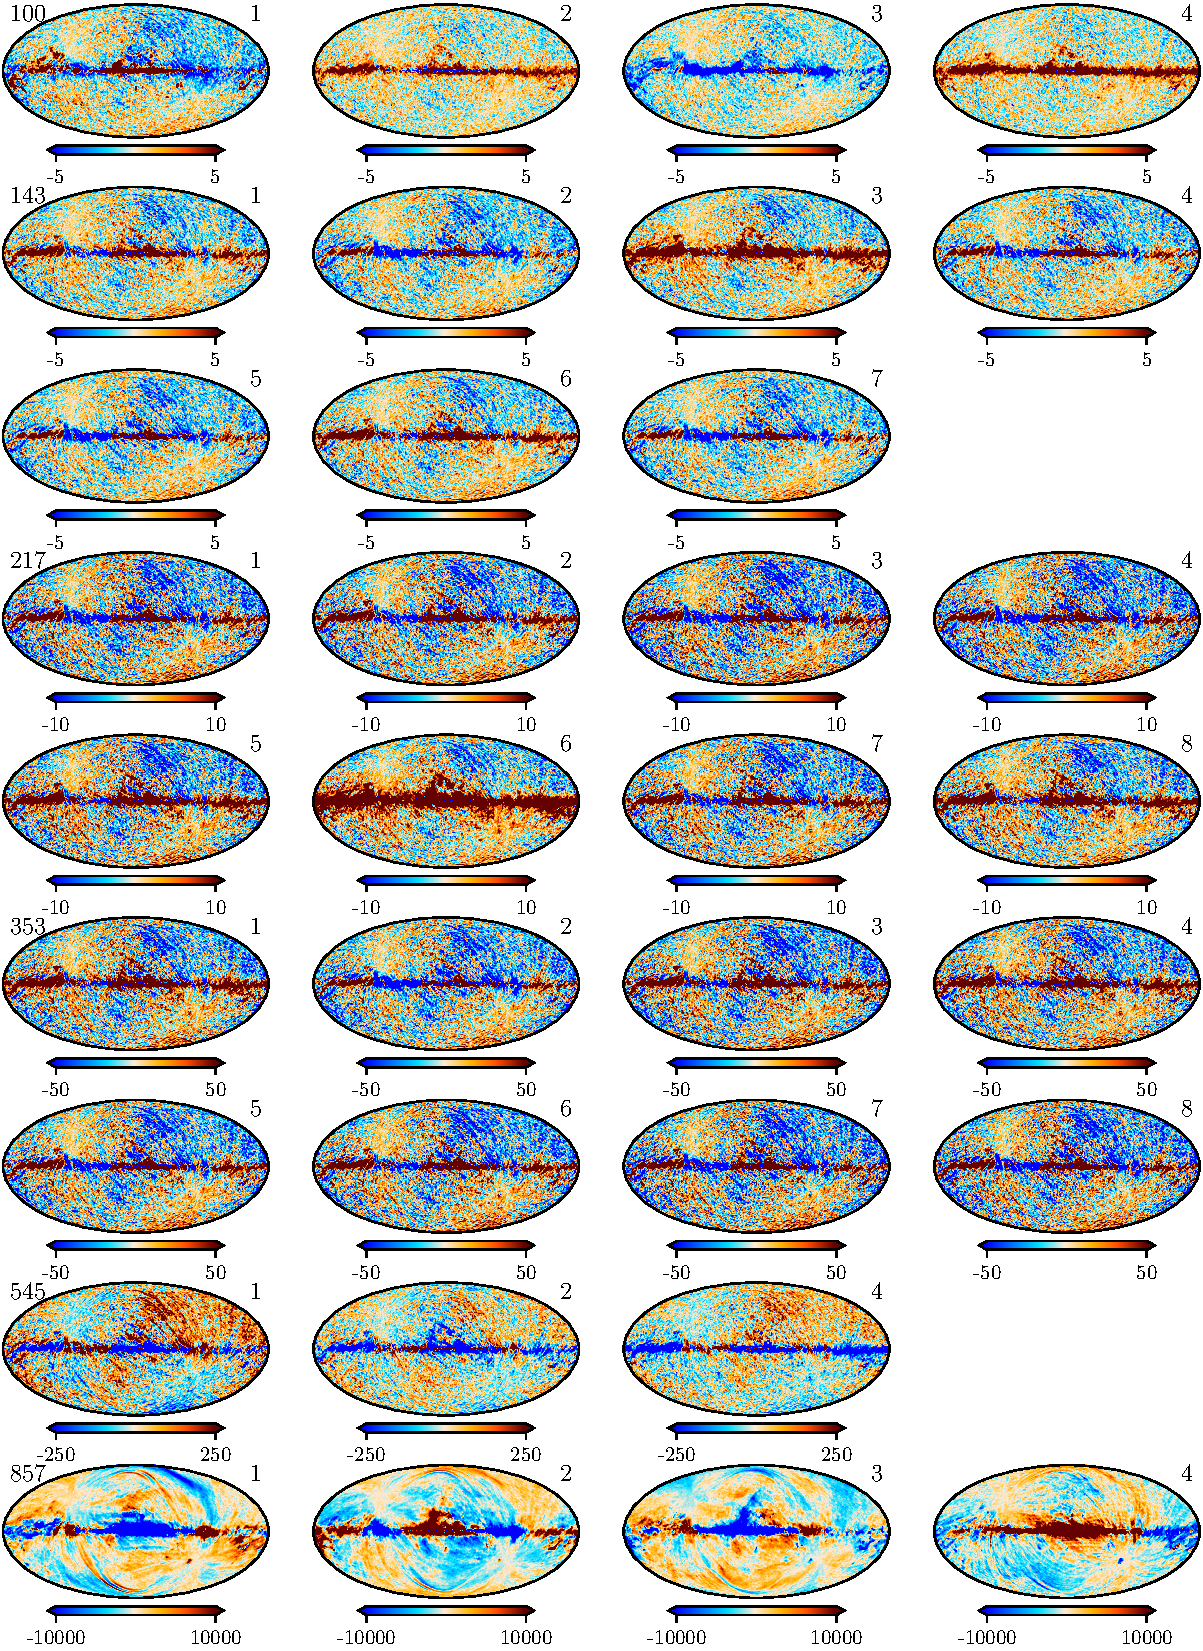
\includegraphics[width=\textwidth]{figures/residuals_plotres.pdf}
\captionof{figure}{Residuals (Data minus model) for the \planck\ HFI bands. Units are in $\mu K_\mathrm{CMB}$. The residuals hint at some uncorrected zodiacal light along the ecliptic plane, as well as potentially some offsets to the gain of the 545 channels.}
\label{fig:residuals}
\end{minipage}


We can see the fidelity of the sky model by looking at the difference between the data and the model at each of the bands (see \cref{fig:residuals}). The residuals indicate potential for improvement to the modelling of the zodiacal light, as well as improvements to the 545~GHz gain. The incredibly low residuals in the 100, 143, 217 and 353~GHz maps demonstrate the success of this model. 

% \clearpage

\section{Grid search tests}
\label{app:GridSearchTests}

\noindent\begin{minipage}{\textwidth}
\vspace*{-3mm}

\centering
\hspace*{1.5cm}\includegraphics[width=0.8\textwidth]{figures/hotDust_cold_Grid_v2.pdf}
\captionof{figure}{Hot dust amplitudes for varying $T_\mathrm{c}$ and $\beta_\mathrm{c}$ values with all other grid parameters set to the fiducial values as recorded in \cref{tab:SEDs}. The center panel is the fiducial map. The corresponding cold dust maps ratios can be seen in \cref{fig:cold_cold_dust_set2}.}
\label{fig:cold_hot_dust_set}

\centering
\hspace*{1.5cm}\includegraphics[width=0.8\textwidth]{figures/coldDust_cold_Grid_ratio_v2.pdf}
\captionof{figure}{Monopole subtracted ratio of the cold dust amplitudes compared to the fiducial value (central panel) for varying $T_\mathrm{c}$ and $\beta_\mathrm{c}$. The corresponding hot dust maps can be seen in \cref{fig:cold_hot_dust_set}.}
\label{fig:cold_cold_dust_set2}
\end{minipage}


\begin{figure*}[t]
    \centering
    \includegraphics[width=0.85\linewidth]{figures/coldDust_hot_Grid_v2.pdf}
    \caption{Cold dust amplitudes for varying $T_\mathrm{h}$ and $\beta_\mathrm{h}$ values with all other grid parameters set to the fiducial values as recorded in \cref{tab:SEDs}. The central panel is the fiducial map. The corresponding hot dust maps ratios can be seen in \cref{fig:hot_hot_dust_ratio}.}
    \label{fig:hot_cold_dust_set}

    \centering
    \includegraphics[width=0.85\linewidth]{figures/hotDust_hot_Grid_ratio_v2.pdf}
    \caption{Monopole subtracted ratio of the hot dust amplitudes compared to the fiducial value (central panel) for varying $T_\mathrm{h}$ and $\beta_\mathrm{h}$. The corresponding cold dust maps can be seen in \cref{fig:hot_cold_dust_set}}
    \label{fig:hot_hot_dust_ratio}    
\end{figure*}

\begin{figure*}[t]
    \centering
    \includegraphics[width=0.85\linewidth]{figures/hotDust_near_Grid_v2.pdf}
    \caption{Hot dust amplitudes for varying $T_\mathrm{near}$ and $\beta_\mathrm{near}$ values with all other grid parameters set to the fiducial values as recorded in \cref{tab:SEDs}. The center panel is the fiducial map. The corresponding cold dust maps can be seen in \cref{fig:near_cold_dust_set}. }
    \label{fig:near_hot_dust_set}

    \centering
    \includegraphics[width=0.85\linewidth]{figures/coldDust_near_Grid_v2.pdf}
    \caption{Cold dust amplitudes for varying $T_\mathrm{near}$ and $\beta_\mathrm{near}$ values with all other grid parameters set to the fiducial values as recorded in \cref{tab:SEDs}. The central panel is the fiducial map. The corresponding hot dust maps can be seen in \cref{fig:near_hot_dust_set}.}
    \label{fig:near_cold_dust_set}
\end{figure*}


We plot several of the maps from the grid search in \cref{sec:results}. Since the \Ha\ dust and nearby dust are templates they do not change by eye (only scaling by a set factor for each frequency given a set of $T,\beta,a$) so they are not plotted here. Thus, we plot the amplitudes of the cold and hot dust for each of the grid points. We show a sample for each of the grids in \cref{fig:SEDGridContours} with the central map the fiducial point and varying the spectral index along the vertical axis and the temperature along the y-axis. 

\subsection{Cold dust}
As can be seen in \cref{fig:SEDGridContours}, there is an unphysical space mapped by the hottest and highest spectral indices in the cold dust grid. This corresponds to large over-subtraction and negative areas in the hot dust amplitudes as can be seen in \cref{fig:cold_hot_dust_set}. When shifting the $T_c$ and $\beta_c$, we find the shape of the amplitude maps is visually similar to the fiducial map (see \cref{fig:dust_figures}), so we show the monopole subtracted ratio of the grid position to the fiducial value in \cref{fig:cold_cold_dust_set2}. 


\subsection{Hot dust}
Similar to with the cold dust, in \cref{fig:SEDGridContours}, there is an unphysical space mapped by the coldest and lowest spectral index in the hot dust grid. This corresponds to large over-subtraction and negative areas in the cold dust amplitudes as can be seen in \cref{fig:hot_cold_dust_set}. Similar to the cold dust, when shifting the $T_h$ and $\beta_h$ we find the shape of the amplitude maps is visually similar to the fiducial map (see \cref{fig:dust_figures}), so we show the monopole subtracted ratio of the grid position to the fiducial value in \cref{fig:hot_hot_dust_ratio}.


\subsection{Nearby Dust}
The nearby dust was found to have unphysical regions banded both by the cold dust amplitudes and the hot dust amplitudes. We additionally aimed to minimize correlations between the cold and nearby, and hot and nearby, dust, such that the dust population described by the nearby dust was an independent dust component. For regions with lower $\beta_\mathrm{near}$ and lower $T_\mathrm{near}$ the cold dust starts to behave unphysically and this corresponds also to a higher correlation between the nearby dust and the hot dust (visible in the lower left panels of \cref{fig:near_hot_dust_set}). 
Conversely, for regions with higher $\beta_\mathrm{near}$ and higher $T_\mathrm{near}$ the hot dust starts to behave unphysically and this corresponds also to a higher correlation between the nearby dust and the cold dust (as can be seen by eye in the upper right panels of \cref{fig:near_cold_dust_set}). 

\subsection{\texorpdfstring{H$\alpha$}{Ha} dust}
The parameter space explored for the \Ha\ correlated dust was shown to have a very flat $\chi^2$ profile, and minimal changes to the hot and cold dust amplitudes and correlations. Since there is no perceivable difference, then, in the cold and hot dust amplitudes during the grid search, we do not include those plots here. As a reminder, we chose to take the DIRBE fit values from \cite{CG02_05} for our fiducial values since the HFI have so little control of this dust component and as we expect the DIRBE bands to have better control of these SED parameters. 

% \clearpage

\section{Thermal dust map characterization}
\label{app:dustCharacterization}
We compare the fraction of each dust component contributing to the total in \cref{fig:dustFrac}. As the \Ha\ dust is a dust extinction, with negative amplitude, it contributes a negative fraction, and it is the smallest contributor to the total. The nearby dust dominates outside the plane of the galaxy (which is to be expected, since further dust will be closer to the Galactic plane due to geometry). The hot dust is clustered nearby the galactic center and shows some anti-correlation with the \Ha\ dust. Finally, the cold dust is dominant in the Galactic plane further from the Galactic center. This further cements the notion that this updated dust model is more physical motivated than previous models, tracing known physical regions within the Milky Way Galaxy. 
\begin{figure*}[h]
    \centering
    \includegraphics[width=0.9\linewidth]{figures/dustFrac_plcmap.pdf}
    \caption{Average dust from each component contributing to the total dust signal. }
    \label{fig:dustFrac}
\end{figure*}



\end{document}
